\chapter{Results}
\label{chap:results}


\section{Hyperparameter gridsearch}

The extended search grid for the hyperparameters of the retrained SMILES models, along with the results from the gridsearch of MassSpecGym, can be found in table \ref{tab:gridsearch}.
The hyperparameter combination for which the trained model has lowest validation loss is denoted in bold.

\begin{table}[h]
	\caption{
		SMILES transformer, Gridsearch MassSpecGym vs Gridsearch from this Thesis (lowest validation loss models in bold)
	}
    \resizebox{\textwidth}{!}{
	\begin{tabular}{p{6cm}W{c}{4cm}W{c}{4cm}}
		\toprule
                \textbf{Hyperparams} & \textbf{MassSpecGym} & \textbf{Thesis Gridsearch} \\
            \midrule
                Learning Rate & $\mathbf{3\cdot 10^{-4}}, 1\cdot 10^{-4}, 5\cdot 10^{-5}$ & $1\cdot 10^{-3}, 3\cdot 10^{-4}, \mathbf{1\cdot 10^{-4}}$\\
                Batch Size & $512, \mathbf{1024}$ & $\mathbf{512}, 1024, 2048$ \\
                $n$ predictions & $\mathbf{10}$ & $\mathbf{10}$ \\
                Transformer hidden dimensionality & $\mathbf{256}, 512$ & $\mathbf{128}, 256, 512$ \\
                Number of attention heads & $\mathbf{4}, 8$ & $2, 4, \mathbf{8}$ \\
                Number of encoding layers & $\mathbf{3}, 6$ & $\mathbf{2}, 3, 4$ \\
                Number of decoding layers & $\mathbf{4}$ & $2, 3, \mathbf{4}$ \\
		\midrule
	\end{tabular}}
	\label{tab:gridsearch}
\end{table}

By retraining with the extended search grid, several models were found that outperformed the retrained model with the best hyperparameter combination from MassSpecGym, when comparing validation loss.
Note that the number of predictions is kept constant as this does not influence the loss.
The hyperparameters from the model with the lowest validation loss differ greatly from the retrained model from MassSpecGym. % 3 keer from?
Because the loss function does not accurately describe the model's ability to predict de novo molecules from \ac{MS/MS},
a naive sampler (that just iteratively samplers from the model's output distribution) was used to predict SMILES on the validation set.
The evaluation of the SMILES predictions from both models using this sampler can be found in figure \ref{fig:gridsearch_vs_paper}.
The MCES distance on the SMILES and tanimoto similarity on the converted fingerprints are calculated in the strict (top-1) and more relaxed (top-10) settings.

\begin{figure}[h]
    \centering
    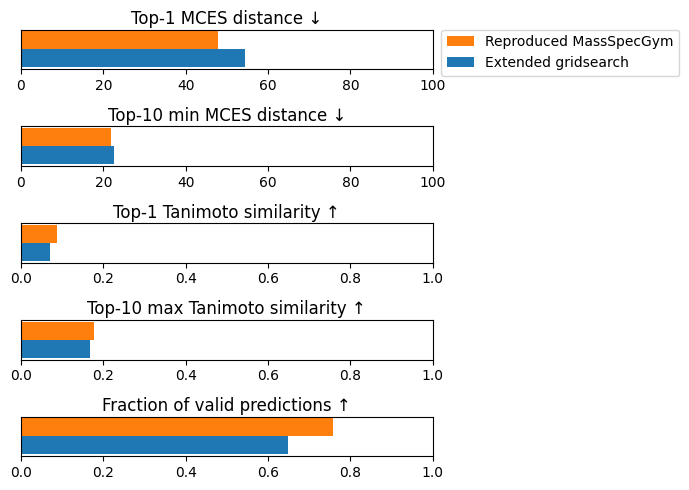
\includegraphics[width=0.6\textwidth]{figures/results/gridsearch_vs_paper.png}
    \caption{Performance comparison between the retrained SMILES model from the MassSpecGym paper versus the lowest validation loss SMILES model from the gridsearch, evaluated on the validation set}
    \label{fig:gridsearch_vs_paper}
\end{figure}

The top-1 and top-10 exact match accuracy for both models is (close to) zero.
Even though the naive sampler adds a bit of randomization by sampling from the output distribution, the retrained SMILES model from MassSpecGym outperforms the model with the lowest validation loss.

A big contributing factor to this performance difference is the fact that the retrained MassSpecGym model is able to predict 10\% more valid SMILES, as invalid SMILES have the maximum MCES distance and zero Tanimoto similarity.
The validity of the SMILES prediction can rely on the sampler and the temperature scaling of the output distribution.
Because only a naive sampler with no temperature scaling was used, it is possible that better performance can be extracted from these models using different samplers and temperature scaling.


\section{Samplers benchmark}

To test how much temperature scaling and different samplers can influence model performance, different samplers were used to predict the validation set of the model with the lowest loss from table \ref{tab:gridsearch}.
For this and all further experiments conducted in this thesis, the Tanimoto similarity is directly correlated to the MCES distance and will thus not be shown in the plots.
All performance differences shown with the MCES distance always show the same relative tanimoto similarities.

Firstly the temperature scaling influence is measured in figure \ref{fig:naive_and_greedy} for the top-1 and top-10 settings.
Because this will influence the randomness the sampler's predictions, a simple greedy sampler that always predicts the most likely token is shown as a deterministic baseline.
This sampler will always predict the same SMILES and can thus only be top-1 evaluated.

\begin{figure}[h]
    \centering
    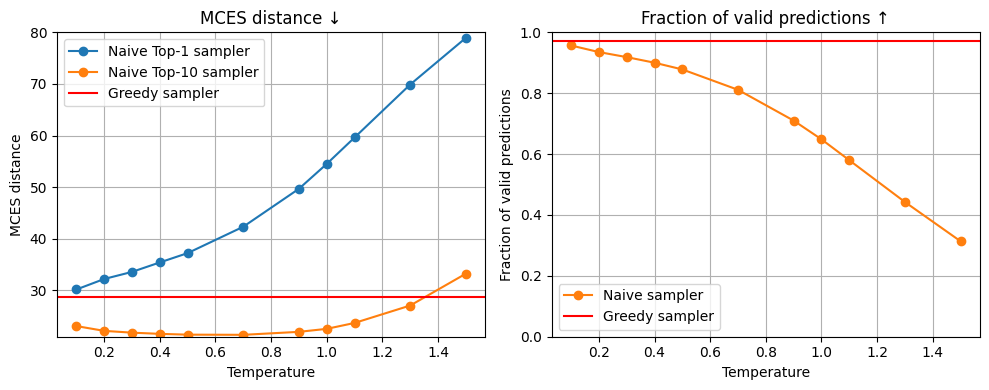
\includegraphics[width=1.0\textwidth]{figures/results/samplers/naive_and_greedy.png}
    \caption{Evaluation of the naive and greedy sampler on the validation set}
    \label{fig:naive_and_greedy}
\end{figure}

From figure \ref{fig:naive_and_greedy}, it is clear that the naive sampler performs poorly when only one prediction is evaluated (top-1).
Increasing the randomness (by increasing the temperature) for the top-1 naive sampler, only worsens the MCES distance.
As expected, the top-1 naive sampler MCES distance converges to the greedy sampler's MCES distance as the temperature approaches zero, as extremely low temperatures force the model to only predict the most likely token.

The top-10 naive sampler benefits greatly from its randomness, by performing better than the greedy sampler according to the MCES distance.
It shows to have an optimal temperature around $0.7$, for this SMILES model.
A higher temperature increases the randomness of the sampler too much causing the amount of valid predictions to drop.
A lower temperature starts to force the predictions towards the greedy sampler.
This shows that temperature can indeed influence the sampler's performance.

\subsection{Stochastic Samplers}

The randomness of the naive sampler can be tweaked using samplers such as top-k and top-p (nucleus sampling).
Because the stochastic samplers only benefit from their randomness when evaluating in a top-10 setting, only these results will be shown on the plots.
The temperature has shown to influence performance, therefore, a temperature search was conducted for each sampler with different parameters $k$ or $p$, where the optimal temperature (according to the lowest MCES distance) was selected.
This ensures that only the best results are shown for each the sampler with its parameter.
For completeness, the top-1, along with the temperature search results can be found in the appendix in section \ref{sec:sampler_full_results}.

\begin{figure}[h]
    \centering
    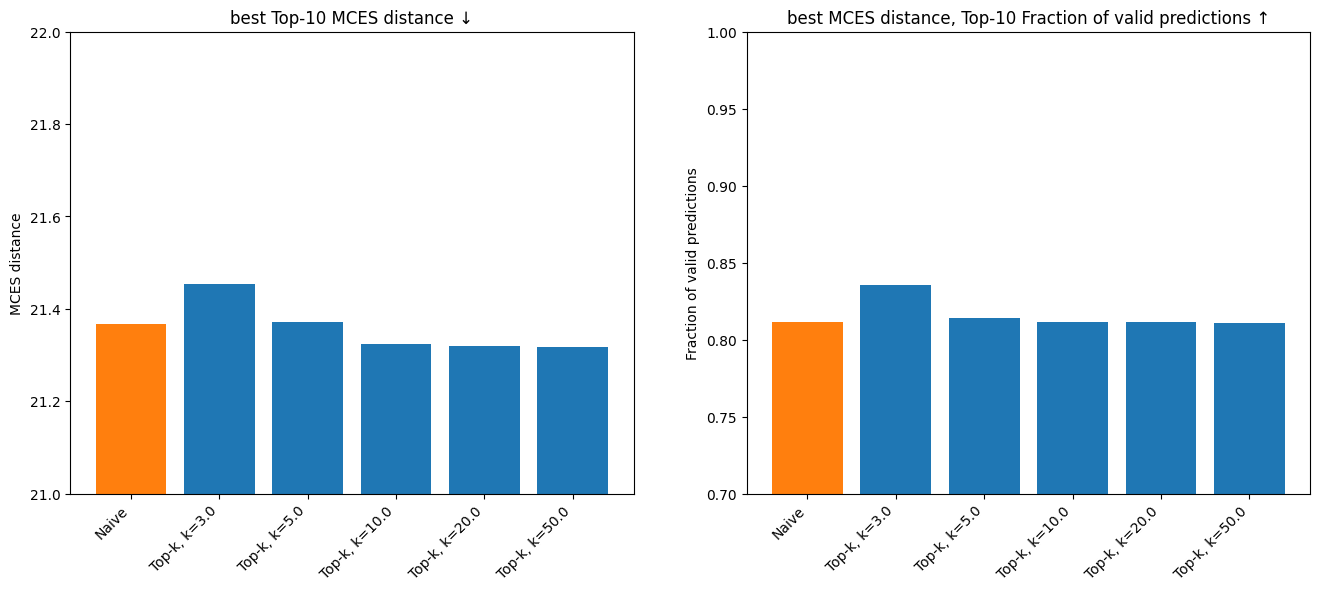
\includegraphics[width=1.0\textwidth]{figures/results/samplers/top-k.png}
    \caption{Evaluation of the (top-10, temperature optimized) top-k sampler and naive sampler on the validation set.}
    \label{fig:top-k}
\end{figure}

Figure \ref{fig:top-k} shows that top-k sampling can slightly improve performance when $k > 5$.
This shows that when the sampler gets forced with a low $k$ it performs slightly worse. 
Note that the y-axis is scaled for visibility, the improvement is very small.

\begin{figure}[h]
    \centering
    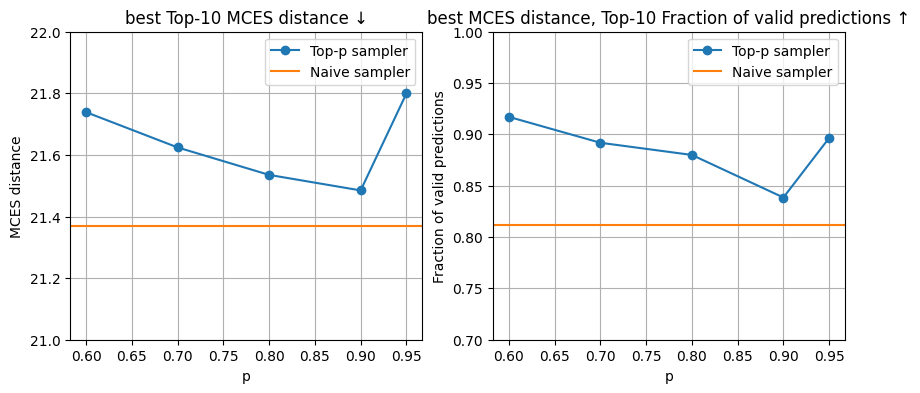
\includegraphics[width=1.0\textwidth]{figures/results/samplers/top-p.png}
    \caption{Evaluation of the (top-10, temperature optimized) top-p sampler and naive sampler on the validation set.}
    \label{fig:top-p}
\end{figure}

With top-k, limiting the randomization seems to slightly improve performance of the sampler, figure \ref{fig:top-p} shows that this does not hold for the top-p sampler.
Overall these randomization limiting samplers do not considerably improve the naive sampler.

The stochastic samplers seem to only benefit from the top-10 evaluation setting where the randomness of the sampler plays to its advantage.
The drawback of this method is the relatively low fraction of valid predictions.
Figure \ref{fig:naive_and_greedy} shows that in the temperature optimum still only $80\%$ of predictions are valid.
Because the top-10 setting only evaluates the best prediction, invalid predictions are not punished as long as there is one valid prediction for a spectrum.
These samplers are for this reason not suited for top-1 evaluation, where every invalid prediction is punished.

\subsection{Deterministic Samplers}

The beam search sampler is another deterministic sampler that improves upon the greedy sampler by increasing its search space to find optimal predictions.
Figure \ref{fig:beam-search} shows its performance for different search space sizes (beam widths).
The length regularization parameter $\alpha$ from the scoring function was also benchmarked for different beam widths but showed to have no influence on performance.
Only when large values were used ($\alpha > 10$), performance tanked to very poor results.
Forcing the sampler to predict longer token sequences with parameter $\alpha$ thus only hinders performance.

\begin{figure}[h]
    \centering
    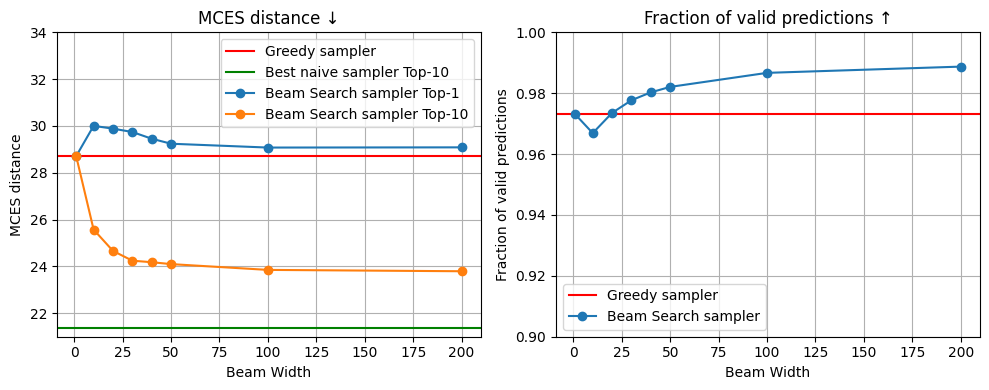
\includegraphics[width=1.0\textwidth]{figures/results/samplers/beam_search.png}
    \caption{Evaluation of the beam search sampler compared to the greedy and naive sampler on the validation set.}
    \label{fig:beam-search}
\end{figure}

Figure \ref{fig:beam-search} shows that the top-1 and top-10 MCES distance for the beam search sampler improves with increased search space as expected.
The spike in MCES distance and fraction of valid predictions on the first data point is because the beam width is 1, meaning it is essentially the same as the greedy sampler.
It outperforms the greedy sampler but does not come close to the best top-10 naive sampler results. 
For the top-1 setting, the performance shows to be worse than the greedy sampler.
This indicates that the scoring function is not optimal for extracting the correct molecular structure, especially with a small search space.
The only metric where the beam search samplers seems to outperform the others is the fraction of valid predictions.

These deterministic sampling methods perform best at predicting valid molecules as the fraction of valid predictions is substantially higher than with the optimal stochastic samplers.
When evaluating in a top-1 setting, where every invalid predictions is punished, these samplers are thus preferred.

Overall, from these results, the greedy sampler seems to perform best for the top-1 setting, while the naive sampler excels in the top-10 setting.


\section{\ac{BPE} as pretraining}

\begin{figure}[h]
    \centering
    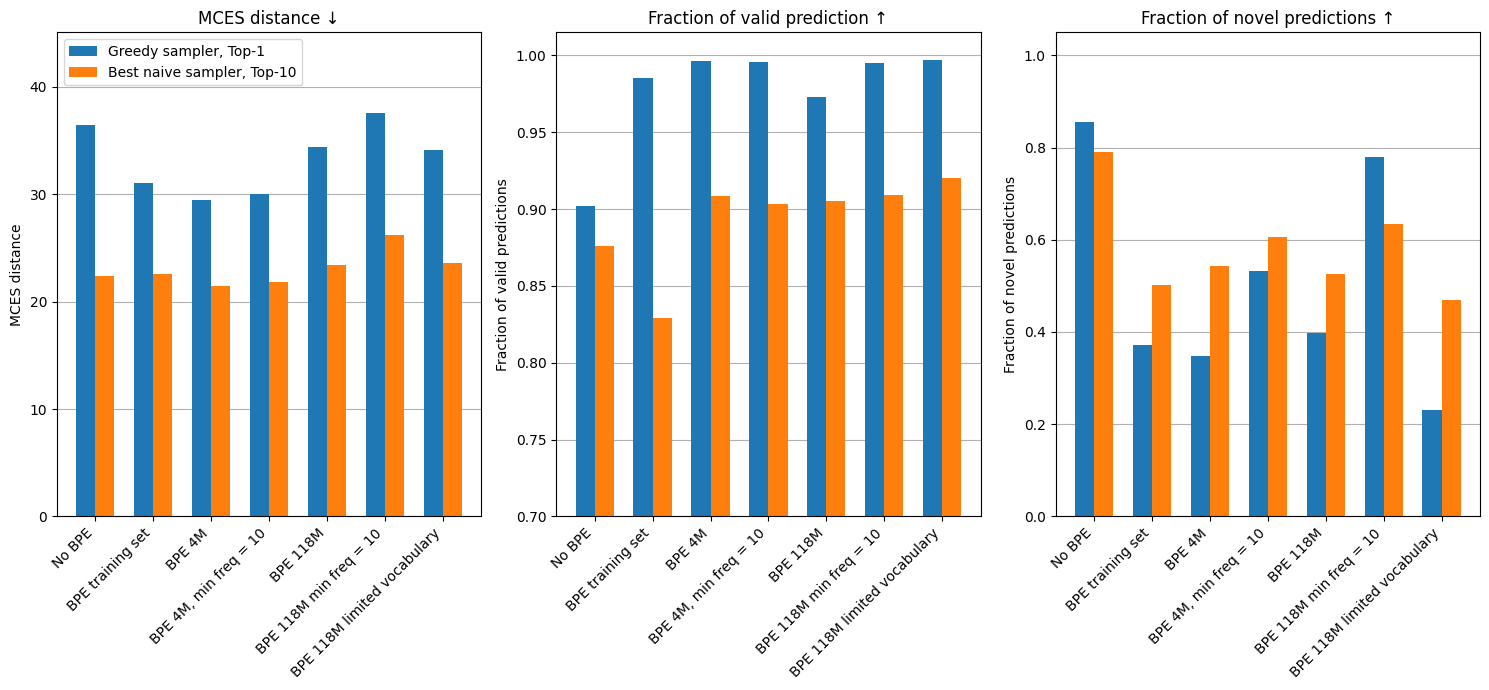
\includegraphics[width=1.0\textwidth]{figures/results/bpe.png}
    \caption{Evaluation on the validation set of SMILES models trained with different tokenizers}
    \label{fig:bpe}
\end{figure}

\section{Augmentation}

\subsection{SMILES augmentation}

\subsection{Spectral augmentation}


\section{Molecular representations benchmark}